% Created 2023-03-23 Thu 18:55
\documentclass[9pt, b5paper]{article}
\usepackage{xeCJK}
\usepackage[T1]{fontenc}
\usepackage{bera}
\usepackage[scaled]{beraserif}
\usepackage[scaled]{berasans}
\usepackage[scaled]{beramono}
\usepackage[cache=false]{minted}
\usepackage{xltxtra}
\usepackage{graphicx}
\usepackage{xcolor}
\usepackage{multirow}
\usepackage{multicol}
\usepackage{float}
\usepackage{textcomp}
\usepackage{algorithm}
\usepackage{algorithmic}
\usepackage{latexsym}
\usepackage{natbib}
\usepackage{geometry}
\geometry{left=1.2cm,right=1.2cm,top=1.5cm,bottom=1.2cm}
\usepackage[xetex,colorlinks=true,CJKbookmarks=true,linkcolor=blue,urlcolor=blue,menucolor=blue]{hyperref}
\newminted{common-lisp}{fontsize=\footnotesize} 
\author{deepwaterooo}
\date{\today}
\title{Unity Zuma 游戏}
\hypersetup{
  pdfkeywords={},
  pdfsubject={},
  pdfcreator={Emacs 28.2 (Org mode 8.2.7c)}}
\begin{document}

\maketitle
\tableofcontents


\section{QQ 龙珠游戏}
\label{sec-1}
\begin{itemize}
\item 是想要写多人版【七人版】QQ 龙珠游戏,在网上搜索C\# 现有的源码版本,找到了这两个,感觉都极不理想,但两个游戏综合,可以合成为一个勉强凑合过得去的小孩子过家家的游戏。
\begin{itemize}
\item 因为是Windows-forms 应用,所以只能在 windows 上运行。但是它有背景贴图
\item Unity 游戏却极为简单
\end{itemize}
\item 源码量极其简单:只有5 个源码文件,但储存小珠的数据结构算法原理还是需要理解一下。 \textbf{源码应该狠简单。打算把它快速读一遍,} 看自己能够在这样一个游戏的基础上如何重新设计实现,或是提升一下至少自己台式机上的运行体验
\item 【学习重点:两个库两个插件】:感觉这个项目最不容易理解和掌握的:反而是背景曲线的生成,与小球延着曲线滚动。要用一个插件,有插件可以帮助生成这些背景图。
\item 【学习重点:两个库两个插件】:有个DoTween 什么动画的,也可以学一下这个插件
\end{itemize}
\subsection{几个最初的游戏体验:}
\label{sec-1-1}
\begin{itemize}
\item 这是自己眼中【小孩子过家家的游戏】:极为简单,会把它稍微改一改,为的是过自己玩过的祖码游戏瘾。
\item 游戏中存在各种各样的 bug, 比如存在同时吐两三粒珠子出来,打到最后,游戏逻辑会崩坏掉,游戏无法继续。。。。。
\end{itemize}

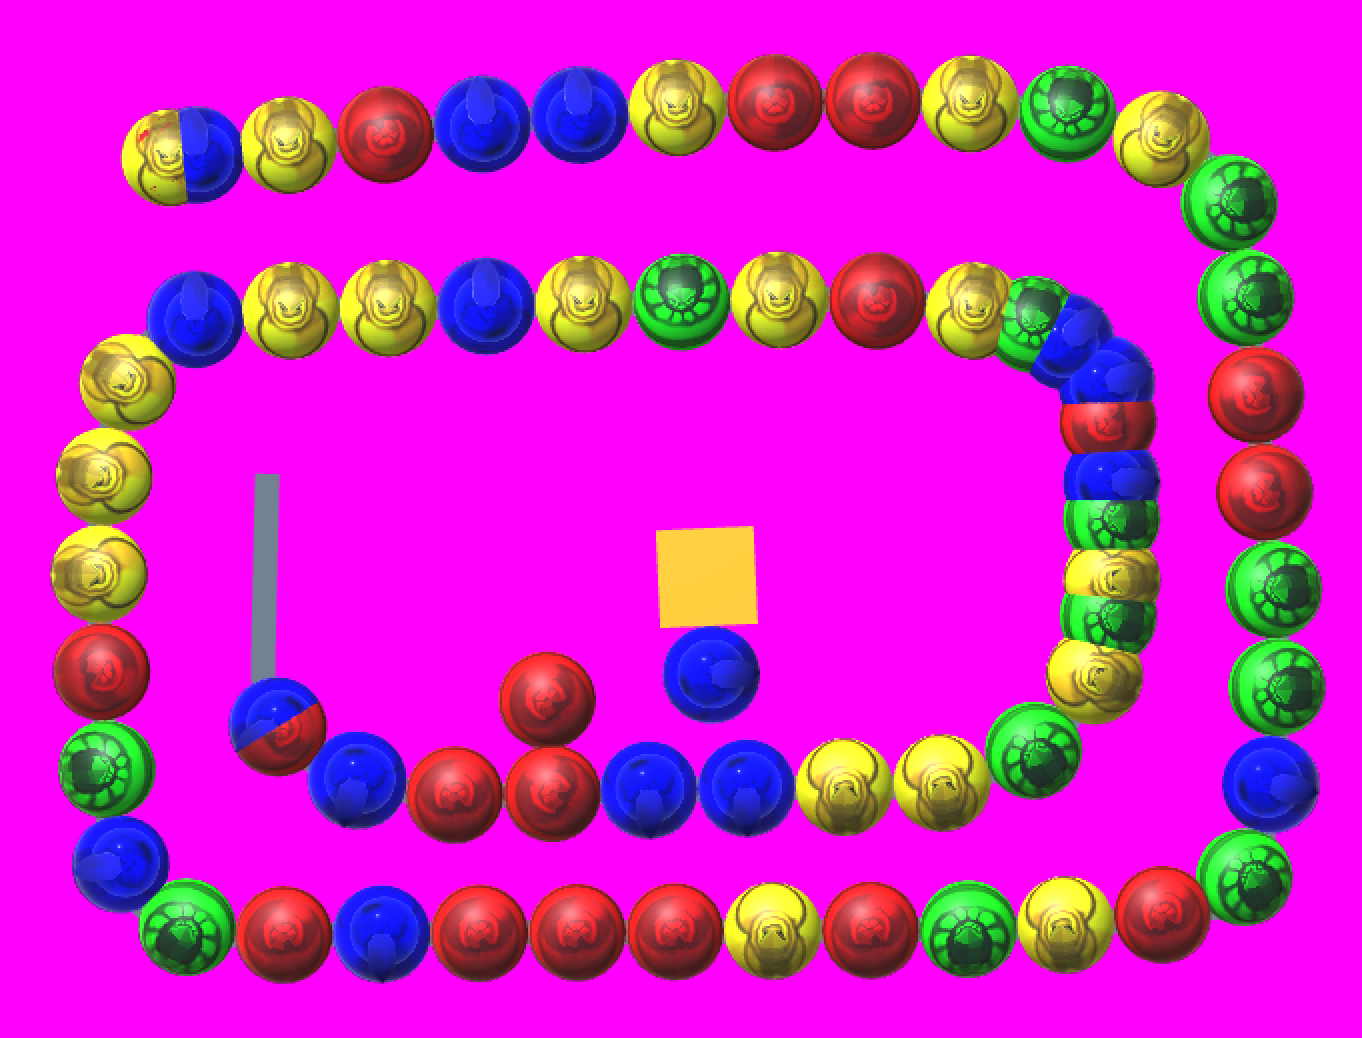
\includegraphics[width=.9\linewidth]{./pic/readme_20230323_112732.png}

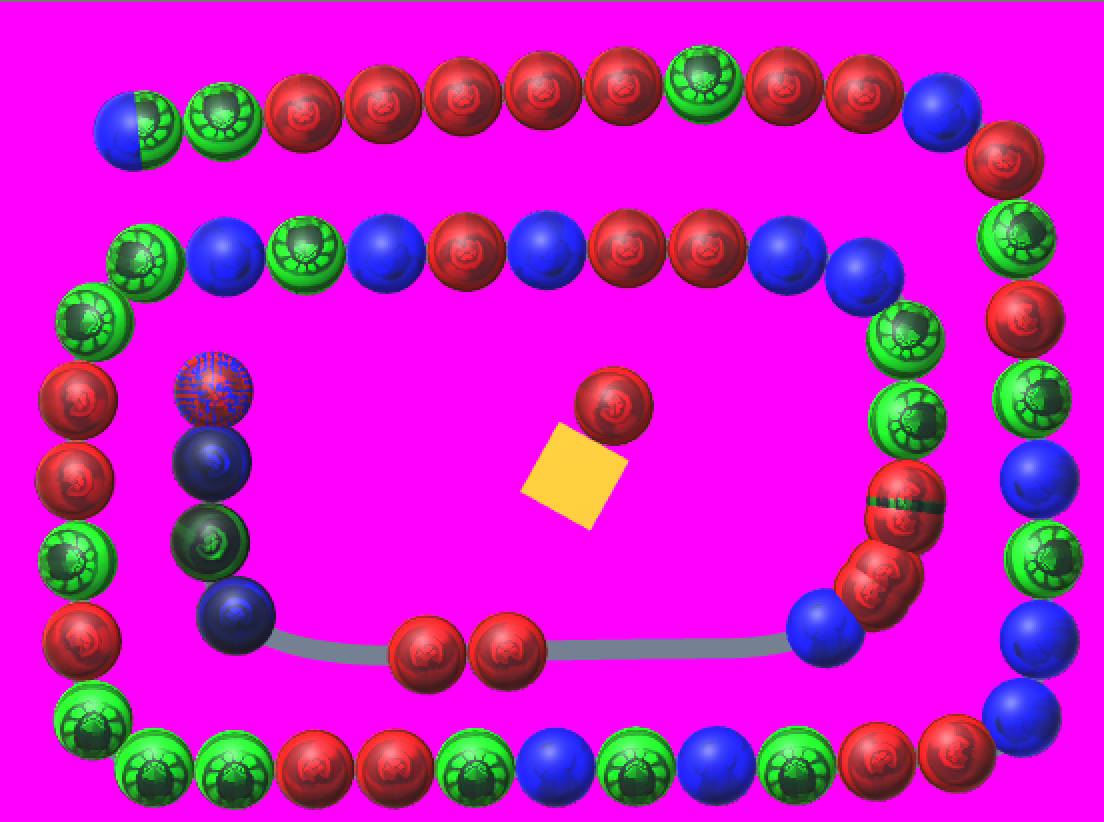
\includegraphics[width=.9\linewidth]{./pic/readme_20230322_223217.png}
\begin{itemize}
\item 增加生成黄色的球儿:它最初随机生成数的范围太少了。填加到 8 种,所有可能性。但是逻辑没有处理完。【亲爱的表哥,活宝妹一定要嫁的亲爱的表哥!!!活宝妹就是一定要嫁给亲爱的表哥!!!】
\end{itemize}

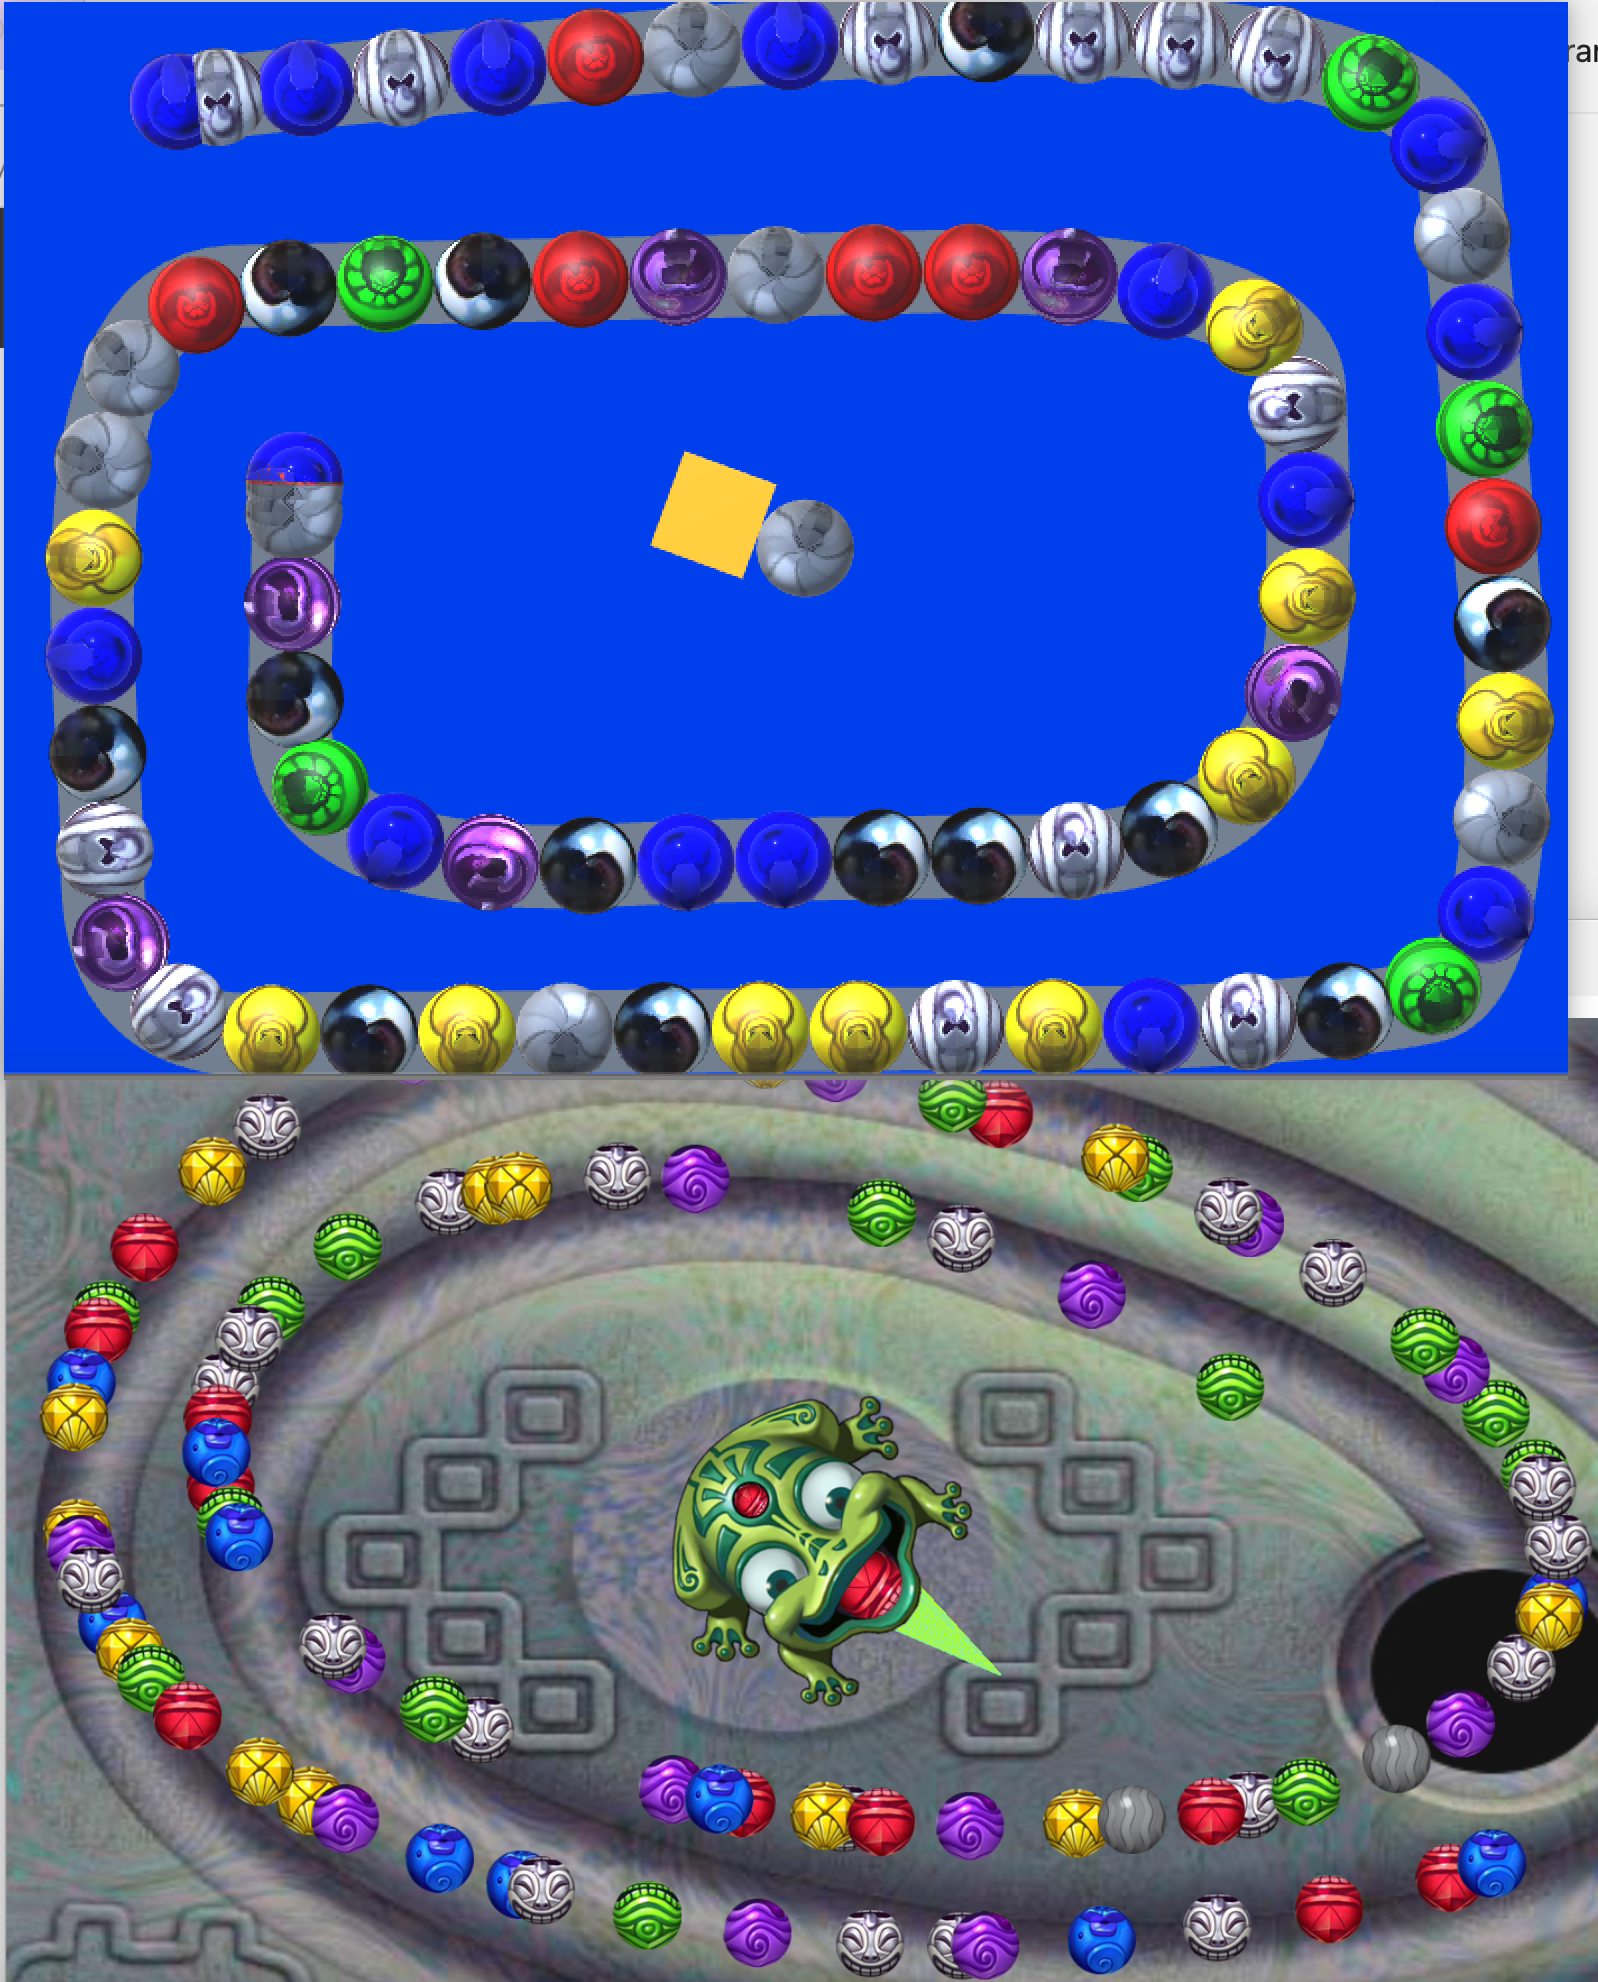
\includegraphics[width=.9\linewidth]{./pic/readme_20230323_185513.png}
\begin{itemize}
\item 小球链表轨道仍然不理想:不真实。需要人们切身感受到的可以放小球的轨道与深度。这里可以参考另一个项目 windows-form 项目:为什么同同样的图片,别人可以沉浸出立体效果,可以作为标尺,也可以参考别人的底层方法。前提是把原理都弄懂。
\item 上面8 种类型没有处理完的逻辑包括:消除的时候不能够区分8 种类型,大概现只能区分一半。
\item 金属碰撞的立体声,与贴图的纹理法线,希望制作出带纹理刻印深度的小球,如同别人想到亲爱的表哥与活宝妹,都会打心底知道,这是一对爱得狠深的情侣,而不是平滑的光滑表面贴图。
\item 视觉声音效果上:鑫龙的头,要一个真正的模型,而不是太无聊的一个立方体。
\item 严重性能问题:与 DoTween 库相互使用,就是同类型不小于2 个,但因为比如碰撞发射球的力度问题,导致小球链表回缩时,不能同步处理消除。这里有逻辑问题、性能问题,需要对游戏逻辑和第三方库都比较理解后才能改得了。现在还不是很懂,仍只是小打小闹地改 bug.
\end{itemize}
\subsection{改装:【可是,它仍是一个小孩子过家家的游戏,有提升,但没有质的飞跃式提升,仍然只是一个经过打扮的小姑娘。。。】}
\label{sec-1-2}
\begin{itemize}
\item 每种球的贴图:用上,就可以看起来好狠多;每种球的大小设置到经曲大小,太小看起来狠奇怪。前面一个游戏不是有很好的贴图吗?直接拿过来借用一下。金龙,也需要一个相对好逼真一点儿的模型。这样视觉上会感觉这个游戏看起来好了狠多;珠子的种类包括: blue, bonus, green purple red stone, white, yellow 共有8 种
\item 需要一点儿特效:消除的时候放放光带点儿闪什么的;消除后往回拉,都能够增加一点儿游戏趣味儿
\item 游戏过程中:方便用户体验的各种菜单:暂停,恢复,游戏进度保存,需要吗,不需要吗?
\item 当背景图多样化,就有了多级关卡。随便整整就可以弄出 27 个关卡来玩儿。。。。。
\item 游戏逻辑不过完整:这条鑫龙,它甚至不能吐出跔多的珠子,不能流出足够多的珠子,游戏逻辑不过完整,仍处在最初的阶段。
\item 把游戏改一改,稍微优化一下:使用对象池什么之类的对小球进行回收。应用直接改成带对象池的 Unity 游戏引擎开发的应用。使用了对像池,应试能够对游戏性能有一定的提升。
\end{itemize}
\subsection{怎么才能把它变成多人网络游戏呢?考虑一下QQ 龙珠到底是如何实现的?}
\label{sec-1-3}
\begin{itemize}
\item 那么就需要添加服务器,需要添加网络模块,需要状态同步
\item QQ 龙珠游戏大家玩得不能再玩了。我应该还需要再想一个什么比较有新意的游戏。
\end{itemize}
\section{Zuma Clone in Unity3D.<br/>}
\label{sec-2}
\begin{itemize}
\item Using Unity 2018.2.8f1.<br/>
\item Asset Credits:
\begin{itemize}
\item Background Material: \url{https://assetstore.unity.com/packages/2d/textures-materials/concrete/clean-concrete-texture-37028}
\item BGCurve: \url{https://assetstore.unity.com/packages/tools/utilities/bg-curve-59043}
\end{itemize}
\end{itemize}
% Emacs 28.2 (Org mode 8.2.7c)
\end{document}